% Metódy inžinierskej práce

\documentclass[10pt,twoside,slovak,a4paper]{article}

\usepackage[slovak]{babel}
%\usepackage[T1]{fontenc}
\usepackage[IL2]{fontenc} % lepšia sadzba písmena Ľ než v T1
\usepackage[utf8]{inputenc}
\usepackage{graphicx}
\usepackage{url} % príkaz \url na formátovanie URL
\usepackage{hyperref} % odkazy v texte budú aktívne (pri niektorých triedach dokumentov spôsobuje posun textu)

\usepackage{cite}
%\usepackage{times}

\pagestyle{headings}

\title{Autopilot\thanks{Semestrálny projekt v predmete Metódy inžinierskej práce, ak. rok 2021/22, vedenie: Vladimír Mlynarovič}} % meno a priezvisko vyučujúceho na cvičeniach

\author{Samuel Švec\\[2pt]
	{\small Slovenská technická univerzita v Bratislave}\\
	{\small Fakulta informatiky a informačných technológií}\\
	{\small \texttt{xsvecs@stuba.sk}}
	}

\date{\small 6.11.2021} % upravte



\begin{document}

\maketitle

\begin{abstract}
Tento článok sa bude venovať histórií a softvérovom fungovaní autopilota v lietadlách a taktiež v automobilovom priemysle. Rozoberie aj aktuálne chyby v softvéroch, ktoré môžu ovplyvniť spoľahlivosť a bezpečnosť autopilota a tým aj zastaviť používanie daného softvéru.
\end{abstract}

Kľúčové slová: autopilot, história, softvér, Tesla, aplikácie

\section{Úvod}

Autopilot nie je v dnešnej dobe nový pojem. S autopilotom sa vieme stretnúť aj v našom bežnom živote, a to napríklad v leteckej či cestnej doprave. V oblasti automobilového priemyslu však nie je dostatočne autopilot využívaný. V súčasnej dobe niekoľko popredných firiem pracuje na vytvorení dokonalého automobilového autopilota, ako napríklad Tesla. Prvý autopilot existuje už vyše sto rokov. Náznaky autonómneho letu pri lietadlách a autonómnej jazdy sú však ešte ďaleko. Jeden z problémov, ktorý bol naznačený v úvode, je podrobnejšie vysvetlený v častiach\ref{ALD} a \ref{PAVAZ}.
Ďalej je to rozvinuté v častiach\ref{ARDAA} a \ref{chyby}


\section{Autopilot v leteckej doprave} 

\subsection{História autopilota v letectve} \label{ALD}

Autopilot je technický systém, ktorý je počas prevádzky schopný zastúpiť človeka v riadení ovládaného objektu bez ďalšej ľudskej asistencie. Historicky prvý funkčný autopilot bol zostrojený v roku 1912 Lawrencom Sperrym, predstavený však bol verejnosti prvý raz až v roku 1914 a uvedený do prevádzky v lodnej doprave.\cite{HistoryAutopilot} Na obr.~\ref{f:obr2} môžeme vidieť vynálezcu Lawrenca Sperryho.

\begin{figure*}[tbh]
\centering
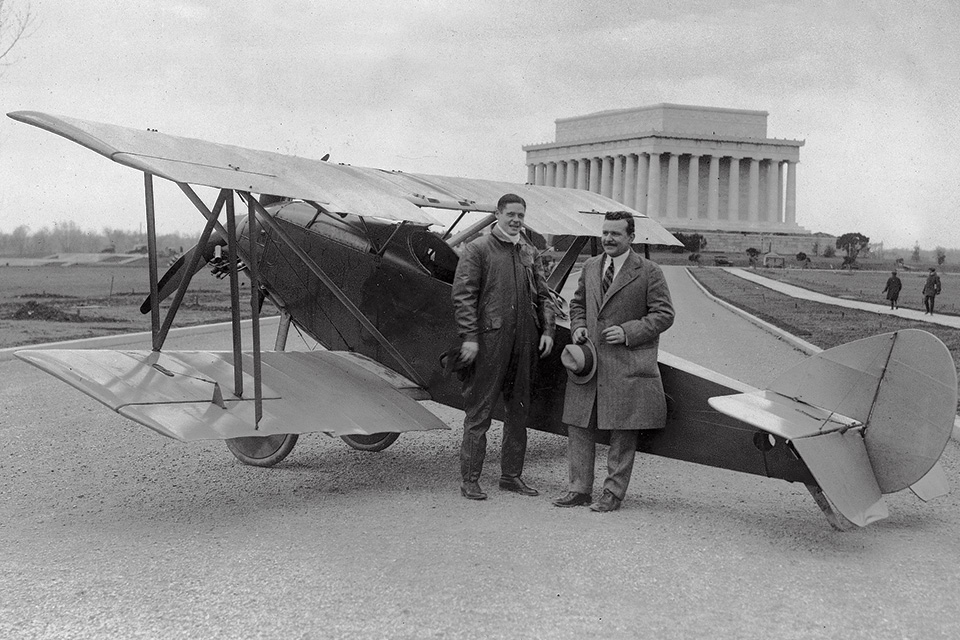
\includegraphics[scale=0.30]{obr2.jpg}
\caption{Lawrence Sperry (naľavo) - prvý funkčný autopilot}
\label{f:obr2}
\end{figure*}

\subsection{Autopilot v lietadlách} \label{AVL}
V letectve sa často stretávame s pomenovaním AFCS.\footnote{Automatic Flight Control Systems - automatické systémy riadenia letu}Tieto systémy sú univerzálne používané v komerčnom letectve. Rozsiahle uplatnenie nachádzajú aj vo vojenskom a všeobecnom letectve, ale koncepcia voľného letu, v rámci ktorej bude v budúcnosti prebiehať plne automatický let, je v podstate zameraná na zníženie preťaženia dýchacích ciest, čo je situácia, ktorá ovplyvňuje najmä komerčné letectvo. Hoci lietadlá všeobecného letectva wm musia tiež pracovať v prostredí voľného letu, väčšina týchto lietadiel má buď iba manuálne riadiace systémy, alebo je inštalácia AFCS len základná.\cite{JenieAFCS}

Hlavným účelom použitia AFCS je do určitej miery automatizovať lietanie lietadla, aby sa znížila pracovná záťaž pilotov (zvyčajne v určitej kritickej fáze letu), aby sa zachovala bezpečnosť letu. Čoraz častejšie sa AFCS používajú aj na zlepšenie základných letových vlastností lietadla (napr. na zabezpečenie dynamickej stability, aj keď bolo lietadlo navrhnuté ako staticky nestabilné), alebo na overenie základných výkonov lietadla v niektorých atmosférických podmienkach. Na dosiahnutie plne automatického letu bude potrebné, aby sa dosiahlo niekoľko dôležitých technologických a operačných systémových vývojov, ale vždy, keď sa to podarí, výsledný plne automatický systém bude fungovať prostredníctvom už vyvinutého AFCS.\cite{McLeanAFCS}

\section{Autopilot v automobiloch}

V následujúcej kapitole bude opísaný vývoj autonómnej jazdy v plne elektrických autách značky Tesla až po súčastnosť.

\subsection{Počiatky autopilota v automobiloch značky Tesla} \label{PAVAZ}

\emph{text bude pridaný vo finálnej verzií}

\subsection{Tesla Autopilot v dnešných dňoch}

\emph{text bude pridaný vo finálnej verzií}

\section{Adaptívne riadenie distribuovaných aplikácií autopilota} \label{ARDAA}

Aj keď sa programovacie modely aj paralelné počítačové systémy naďalej rýchlo vyvíjajú, väčšina analýz výkonnosti zostáva založená na procese vyvinutom pred viac ako štyridsiatimi rokmi:

\begin{enumerate}
\item \emph{Aplikačné prístrojové vybavenie} - Aplikačný kód môže byť vybavený nástrojmi automaticky alebo manuálne vložením volaní do rutín knižnice nástrojov. Počas následného vykonávania knižnica nástrojov zaznamenáva príslušné údaje o výkone, vrátane počtu a časov vykonávania procedúr, slučiek a základných blokov.
\item\emph{Extrakcia údajov o výkone} - Po inštrumentácii sa zachytia údaje o výkone z jedného alebo viacerých vykonávaní programu. V ideálnom prípade tieto spustenia zahŕňajú vstupné údaje a výpočtové zdroje typické pre tie, ktoré sa vyskytujú v produkčnom prostredí.
\item\emph{Analýza a vizualizácia} - Po následnom spracovaní sa údaje o výkone vizualizujú a analyzujú, aby sa identifikovali úzke miesta výkonu aplikačného programu (napr. pomocou textových profilovacích nástrojov alebo vizualizačných systémov ako AIMS  alebo Pablo)
\item\emph{Optimalizácia aplikácie} - Na základe merania a analýzy sa buď program upraví tak, aby sa zmiernili vnímané úzke miesta, alebo sa prispôsobia pravidlá runtime systému tak, aby lepšie zodpovedali požiadavkám na zdroje programu. \cite{SoftverAutopilot}
\end{enumerate}

\subsection{Softvérové komponenty autopilota}

Oddelením merania výkonu, riadenia a rozhodovania umožňuje Autopilot systémovým dizajnérom nahradiť softvérové rozhodovacie postupy vizualizáciou v reálnom čase a interaktívnym riadením, keď rýchlosť zmien pripúšťa ľudskú kontrolu.

Akýkoľvek adaptívny riadiaci systém musí monitorovať príslušné stavy systému, určiť, aké zmeny sú potrebné, a tieto zmeny realizovať, aby sa splnili požadované ciele. Aby sa dynamicky optimalizovalo správanie aplikácií a behu systému pre distribuované výpočtové siete, systém adaptívneho výkonu s uzavretou slučkou musí zahŕňať
niečo z nasledujúceho:

\begin{itemize}
\item \emph{Distribuované senzory výkonu} - dokážu zachytiť údaje o výkone aplikácií a systému a generovať popisy požiadaviek na zdroje a metriky výkonu
\item \emph{Softvérové ovládače} - môžu povoliť a konfigurovať správanie aplikácií a zásady správy zdrojov
\item \emph{Rozhodovacie procedúry} - ako lokálne, tak aj globálne, na výber politík správy zdrojov a aktivovanie akčných členov na základe pozorovaných požiadaviek na zdroje aplikácií a systémových odoziev zachytených senzormi výkonu.
\item \emph{Rozhodovacie mechanizmy} - využívajú údaje z distribuovaných senzorov na vyváženie často protichodných optimalizačných cieľov
\item \emph{Distribuované menné servery} - podporujú registráciu vzdialených senzorov a akčných členov a požiadavky na senzory a akčné členy založené na vlastnostiach vzdialených klientov
\item \emph{Klienti senzorov a akčných členov} - interagujú so vzdialenými senzormi a akčnými členmi, monitorujú dáta senzorov a vydávajú príkazy akčným členom \cite{SoftverAutopilot}
\end{itemize}

\section{Chyby autopilota} \label{chyby}

V tejto kapitole budú opísané chyby autopilota.

\section{Zhrnutie}

\bibliography{literatura}
\bibliographystyle{plain} 
\end{document}